\documentclass{article}
\usepackage{fullpage}
\usepackage{indentfirst}
\usepackage{amsmath}
\usepackage{amsfonts}
\usepackage{pifont}
\usepackage{array}
\usepackage{tipa}
\usepackage{tikz}
\usepackage{tikz-qtree}
\usetikzlibrary{matrix}
\usepackage{gb4e}
\noautomath
\usepackage[backend=bibtex8]{biblatex}
\addbibresource{references.bib}
\newcommand{\Y}{$\checkmark$}
\newcommand{\N}{\ding{55}}
\title{QP 2 Update: 7/9}
\author{Chris Oakden}
\begin{document}
\maketitle
There are two main goals for this update:
\begin{exe}
\ex
\begin{xlist}
	\ex Widen the empirical scope of right-dominant (non-domain-wide spreading) sandhi patterns and characterize them as ISL or OSL.
	\ex Develop a preliminary definition of the ``contour strictly-local" class of stringsets.
\end{xlist}
\end{exe}
\section{Right-dominant sandhi patterns}
In this section, we will look at more right-dominant sandhi patterns in various dialects, and offer an SL function characterization in terms of ISL and OSL functions. This will include disyllabic and trisyllabic patterns.
\subsection{Disyllabic sandhi}
In an analysis of directionality in sandhi processes, Zhang (2007) identifies canonical cases of right-dominant disyllabic sandhi patterns\cite{zhang2007}. Many of these are cases of contrast neutralization in leftmost position. One example is the Wu dialect Wuyi \cite{fu1984}; in a six-tone system (in phonetic notation: /24, 213, 53, 31, 55, 13/), leftmost tones neutralize to one of two non-lexical sandhi tones: 
\begin{exe}
\ex
\begin{xlist}
	\ex /24, 213, 53/ $\rightarrow$ \textbf{55} / \underline{\hspace{1em}} T
	\ex /31, 55, 13/ $\rightarrow$ \textbf{11} / \underline{\hspace{1em}} T
\end{xlist}
\end{exe}
Putting aside issues like the ostensible chain shift (/x/ $\rightarrow$ [55]; /55/ $\rightarrow$ [11]), it is clear that Wuyi is a case of right-dominant sandhi with substitution at the syllable level. Lexical tones surface in their sandhi form regardless of which tone follows them. A similar example comes from ``Type B" sandhi in New Shanghai which, surprisingly, is also right-dominant \cite{xuetal1981}:
 \begin{exe}
\ex
\begin{xlist}
	\ex /HL, MH/ $\rightarrow$ \textbf{H} / \underline{\hspace{1em}} T
	\ex /LH/ $\rightarrow$ \textbf{M} / \underline{\hspace{1em}} T
\end{xlist}
\end{exe}
\par
Other dialects neutralize in a more straight-forward fashion, that is, the surface forms have an analog in the input. The Hakka dialect Yudu is a representative example\cite{xie1992}. In non-checked tones, two of five lexical contrasts are lost in initial position.
\begin{exe}
\ex
\begin{xlist}
	\ex /31, 35/ $\rightarrow$ \textbf{31} / \underline{\hspace{1em}} T
	\ex /44, 22/ $\rightarrow$ \textbf{44} / \underline{\hspace{1em}} T
	\ex /42/ $\rightarrow$ \textbf{42} / \underline{\hspace{1em}} T	
\end{xlist}
\end{exe}
\par
Not all neutralization is insensitive to adjacent tones, however. In Zhangping \cite{zhang1983}, a Min dialect, three of the five lexical tones neutralize to either [33] or [55] based on the following tone, while the other two tones have a single sandhi form regardless of environment:
\begin{exe}
\ex \label{zp1}
\begin{xlist}
	\ex /24, 11, 21/ $\rightarrow$ \textbf{33} / \underline{\hspace{1em}} 24, 11, 53; \textbf{55} / \underline{\hspace{1em}} 31, 21
	\ex /31, 53/ $\rightarrow$ \textbf{21} / \underline{\hspace{1em}} T
\end{xlist}
\end{exe}
Abstracting away from certain details, all three patterns are of the canonical right-dominant form. \par
Environment-insensitive neutralization patterns are ambiguous between being ISL and OSL; they make the same predictions. Whether looking at the input or the output, as long as any tone follows within a particular domain, the process will occur. In the Zhangping data, the maps /24, 11, 21/ $\rightarrow$ [33] and /24, 11, 21/ $\rightarrow$ [55] are also arguably both ISL and OSL. Within a disyllabic domain, the rightmost tone will surface identical to its lexical form. This characteristic is what defines ``right-dominant" sandhi patterns. \par
The disyllabic domain is insufficient in characterizing these patterns unambiguously as ISL or OSL. Returning to the Zhangping example, there is no indication of surface forms of /24, 11, 21/ in the environment of a \emph{sandhi} tone ([33], [55], [21]).
\begin{exe}
\ex
\begin{xlist}
	\ex /24, 11, 21/ $\rightarrow$ \textbf{?} / \underline{\hspace{1em}} 33
	\ex /24, 11, 21/ $\rightarrow$ \textbf{?} / \underline{\hspace{1em}} 55
	\ex /24, 11, 21/ $\rightarrow$ \textbf{?} / \underline{\hspace{1em}} 21
\end{xlist}
\end{exe}
The rules as described in (\ref{zp1}) predict /24, 11, 21/ to surface as [55] before a \emph{lexical} /21/ tone; but does the same apply to a (potentially) phonetically-identical \emph{sandhi} form (of the lexical /31, 53/)? If so, this is an argument in support of OSL. The inverse could possible be evidence for ISL. Without strings of size $>$ 2, however, the determination cannot be made.
\subsection{Trisyllabic sandhi}
 Longer strings are required to determine whether certain sandhi patterns can be represented as ISL or OSL functions. Let us begin with strings of length 3. Earlier, we encountered trisyllabic tone sandhi in Tianjin; the three rules which described those processes were argued to be both ISL (for one rule) and OSL (for two other rules). \par
Recent experimental work in Nanjing has yielded characterizations of trisyllabic sandhi in that dialect \cite{Maandli2014}. Production experiment results suggest that trisyllabic sandhi in Nanjing is describable by the same rules which apply in disyllabic domains. The disyllabic rules which the authors use (different from what I have been using in the past) are in (\ref{nj1}), where `q' stands for a checked tone:
\begin{exe}
\ex \label{nj1}
\renewcommand{\arraystretch}{1.5}
\begin{tabular}[t]{|c|l|l|}
\hline
Rule & Input & Output \\
\hline
R1 & F+F & H+F \\
\hline
R2 & L+F & R+F \\
\hline
R3 & R+q & L+q \\
\hline
R4 & H+q & F+q \\
\hline
R5 & q+q & 3+q \\
\hline
R6 & L+L & R+L \\
\hline
\end{tabular}
\end{exe}
In sequences of three syllables, the authors argue that there is a clear ``rightward" directionality at play. Abstracting away from sequences of three checked tone syllables, there are nine patterns of interest:
\begin{exe}
\ex
\renewcommand{\arraystretch}{1.5}
\begin{tabular}[t]{|c|l|l|}
\hline
& Input & Output \\
\hline
1 & F + F + F & \underline{F + F} + F $\rightarrow$ H + \underline{F + F} $\rightarrow$ H + H + F \\
\hline
2 & L + F + F & \underline{L + F} + F $\rightarrow$ R + \underline{F + F} $\rightarrow$ R + H + F \\
\hline
3 & L + L + F & \underline{L + L} + F $\rightarrow$ R + \underline{L + F} $\rightarrow$ R + R + F \\
\hline
4 & R + q + q & \underline{R + q} + q $\rightarrow$ L + \underline{q + q} $\rightarrow$ L + 3 + q \\
\hline
5 & H + q + q & \underline{H + q} + q $\rightarrow$ F + \underline{q + q} $\rightarrow$ F + 3 + q \\
\hline
6 & L + L + L & \underline{L + L} + L $\rightarrow$ R + \underline{L + L} $\rightarrow$ R + R + L \\
\hline
7 & L + R + q & L + \underline{R + q} $\rightarrow$ L + L + q \\
\hline
8 & F + H + q & F + \underline{H + q} $\rightarrow$ F + F + q \\
\hline
9 & L + H + q & L + \underline{H + q} $\rightarrow$ L + F + q \\
\hline
\end{tabular}
\end{exe}
There is a lot to unpack here. Let's begin with lines 1 and 2. Line 1 exemplifies the application of R1. This rule is either ISL or LOSL, but not ROSL, which would predict /FFF/ $\rightarrow$ *FHF (an analog for R6 is apparent in line 6). Two rules apply in line 2, R2 and R1, and application is opaque (counterbleeding). We know already that R1 is not ROSL, so we cannot be sure about R2. What we can be sure of is that, if it is OSL (either right or left), the order of composition is important.
\begin{exe}
\ex
\begin{tabular}[t]{|c|c|c|}
\hline
Input & OSL1 $\circ$ OSL2 & OSL2 $\circ$ OSL1 \\
\hline
L F F & *LHF & RHF \\ 
\hline
\end{tabular}
\end{exe}
If both are ISL, on the other hand, we achieve the same result regardless of order of composition:
\begin{exe}
\ex
\begin{tabular}[t]{|c|c|c|}
\hline
Input & ISL1 $\circ$ ISL2 & ISL2 $\circ$ ISL1 \\
\hline
L F F & RHF & RHF \\ 
\hline
\end{tabular}
\end{exe}
 \par
The same generalization applies to rules R6 and R2 in line 3; order of composition does not matter when both are represented as ISL functions, but does when both are represented as OSL. 
\begin{exe}
\ex
\begin{tabular}[t]{|c|c|c||c|c|}
\hline
Input & ISL6 $\circ$ ISL2 & ISL2 $\circ$ ISL6 & OSL6 $\circ$ OSL2 & OSL2 $\circ$ OSL6  \\
\hline
L L F & RRF & RRF & RRF & *LRF   \\ 
\hline
\end{tabular}
\end{exe}
The pattern emerging from these examples (and in lines 4, 5, and 6) is the so-called ``rightward" mode of application. In terms of SL functions, it means that composition only becomes important when the functions are OSL. The order seems to be one such that the rule which applies on the first and second syllables must be ordered before the one which applies on the second and third syllables.
\par
Lines 7-9 see the application of R3 and R4 on the second and third syllables resulting in more opacity (the rules R1, R2, and R6 are not surface true). Again, this suggests either that R1, R2, and R6 are ISL \emph{or} that an ordering is imposed on their composition as OSL functions, namely, R3 $\circ$ R6, R4 $\circ$ R1, and R4 $\circ$ R2. This leaves us with the following characterizations of the rules as SL functions.
\begin{exe}
\ex
\begin{tabular}[t]{|c|l|l|l|}
\hline
Rule & ISL & LOSL & ROSL \\
\hline
R1 & \Y & \Y (with ordering) & \N \\
\hline
R2 & \Y & \Y (with ordering) & \Y (with ordering) \\
\hline
R3 & \Y & \Y (with ordering) & \Y (with ordering) \\
\hline
R4 & \Y & \Y (with ordering) & \Y (with ordering) \\
\hline
R5 & \Y & \Y (with ordering) & \Y (with ordering) \\
\hline
R6 & \Y & \Y (with ordering) & \N \\
\hline
\end{tabular}
\end{exe}
\par
There is something dissatisfying in this analysis, because it seems the ordering of composition is arbitrary. Or, rather, that the ordering of the rules is specified by the order of the syllables in a trisyllabic sequence (which can be arbitrary). Assuming that all functions are OSL, the following orderings are necessary: 
\begin{exe}
\ex
\begin{xlist}
	\ex OSL2 $\circ$ OSL1 (via line 2)
	\ex OSL6 $\circ$ OSL2 (via line 3)
	\ex OSL3 $\circ$ OSL5 (via line 4)
	\ex OSL4 $\circ$ OSL5 (via line 5)
	\ex OSL6 $\circ$ OSL4 (via line 7)
	\ex OSL1 $\circ$ OSL4 (via line 8)
	\ex OSL2 $\circ$ OSL4 (via line 9)  
\end{xlist}
\end{exe}
Composing these orderings, we have two possible total orders (\ref{or1}):
\begin{exe}
\ex \label{or1}
\begin{xlist}
	\ex OSL6 $\circ$ OSL2 $\circ$ OSL1 $\circ$ OSL3 $\circ$ OSL4 $\circ$ OSL5
	\ex OSL6 $\circ$ OSL2 $\circ$ OSL3 $\circ$ OSL1 $\circ$ OSL4 $\circ$ OSL5
\end{xlist}
\end{exe}
Luckily, none of the orders contradict one another, but the fact remains that a specific order is necessary on the OSL functions while no order is necessary on the ISL functions. Additionally, we are not any closer to categorizing these processes as ISL or OSL definitively (with the exception of R1 and R6). \par
Next time, I will work on trisyllabic sandhi in Chengdu, which is said to be bidirectional \cite{Yan2016}. The crucial data are presented in (\ref{cd1}) and (\ref{cd2}).
\begin{exe}
\ex \label{cd1}
Disyllabic Sandhi \\
\begin{tabular}[t]{|c|l|l||c|l|l|}
\hline
Rule & Input & Output & Rule & Input & Output \\
\hline
R1 & MH.MH & MH.\textbf{M} &  R6 & ML.LM & ML.\textbf{L} \\
\hline
R2 & ML.MH & ML.\textbf{M} & R7 & HM.LM & \textbf{H}.\textbf{L} \\
\hline
R3 & HM.MH & \textbf{H}.\textbf{M} & R8 & LM.LM & LM. \textbf{L} \\
\hline
R4 & LM.MH & LM.\textbf{H} & R9 & HM.ML & \textbf{H}.ML \\ 
\hline
R5 & MH.LM & MH.\textbf{L}& R10 & HM.HM & \textbf{H}.HM \\
\hline
\end{tabular}
\end{exe}

\begin{exe}
\ex \label{cd2}
Trisyllabic Sandhi \\
\begin{tabular}[t]{|c|l|l|l|}
\hline
& Input & Output & ``Directionality" \\
\hline
1 & MH.LM.MH & MH.\textbf{L.M} & R \\
\hline
2 & ML.LM.MH & ML.\textbf{L.M.} & R \\
\hline
3 & HM.LM.MH & \textbf{H.L.M} & R \\
\hline
4 & LM.LM.MH & LM.\textbf{L.M.} & R \\
\hline
5 & MH.MH.MH & MH.\textbf{M.M} & L \\
\hline
6 & ML.MH.MH & ML.\textbf{M.M} & L \\
\hline
7 & HM.MH.MH & \textbf{H.M.M} & L \\ 
\hline
\end{tabular}
\end{exe}
\section{Contour strictly-local stringsets}
What follows is an attempt at a very preliminary definition of (or at least motivation for) the contour strictly-local stringsets (CSL). The core intuition that such a grammar endeavors to capture is the psychological reality of the \emph{tonal category} in Chinese dialects, that is, the Middle Chinese categories \emph{ping}, \emph{shang}, \emph{qu}, and \emph{ru}. Tone categories indicate the abstract representation of tones at the syllable level, and for which (almost) every syllable in Chinese dialects is lexically specified. This level of representation offers a straightforward and consistent characterization of the illicit substructures that trigger sandhi, and is in fact necessary to provide such generalizations; purely melodic representations fail to isolate the environments which trigger sandhi (see earlier updates). At the same time, however, access to the melodic tier is crucial in deriving certain dissimilatory and assimilatory processes and in constraining them. Take, for example, OCP effects for adjacent contours in Tianjin:
\begin{exe}
\ex
\begin{tabular}[t]{|l|l|l|l|l|}
\hline
Input & Output & $\mathtt{cntr(w)}$ & Unattested & $\mathtt{cntr(w)}$ \\
\hline
FF & LF & L.HL & *HF & \textbf{H.H}L \\ 
\hline
RR & HR & H.LH & *LR & \textbf{L.L}H \\
\hline
\end{tabular}
\end{exe}
Dissimilation occurs at the syllabic level to avoid the ill-formed sequences *FF and *RR. Contour simplification further avoids OCP violations at the \emph{melodic} level (*HH and *LL). There is much more to be said about this example, but for our purposes it provides suggestive evidence of the importance of melodic-level representations. More broadly, this question is of interest because it bears on an important debate about whether contours in Chinese dialects are units or sequences of level tones.\par
The basic conceptualization of contour strictly-local grammars is that they isolate syllable-level tonal categories, allowing for abstract representation of level and contour tones alike. Access to the melodic tier is available via some function (essentially the inverse of $\mathtt{cntr(w)}$), transforming tonal categories into their component ``parts", and permitting melody-level constraints. This is schematized below.
\begin{exe}
\ex 
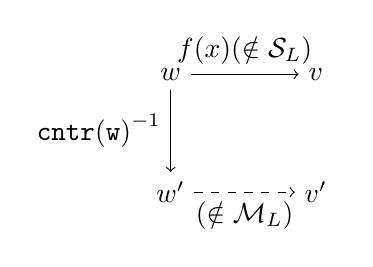
\begin{tikzpicture}[baseline=(m-1-1.base)]
\matrix (m) [matrix of nodes, row sep = 3em] {
$w$ & \hspace{3em} & $v$   \\
$w'$ & \hspace{3em} & $v'$  \\
};
\draw [->] (m-1-1.east) -- (m-1-3.west) node [above, pos=.5] {$f(x) (\notin\mathcal{S}_{L})$};
\draw [->] (m-1-1.south) -- (m-2-1.north) node [left, pos=.5] {$\mathtt{cntr(w)}^{-1}$};
\draw [dashed, ->] (m-2-1.east) -- (m-2-3.west) node [below, pos=.5] {($\notin\mathcal{M}_{L})$};
\end{tikzpicture}
\end{exe}
Above, the mapping $w \mapsto v$ of some input string to some output string occurs via a CSL function, such that the output is in the syllable-level stringset (and therefore not in the illicit substructure grammar specified for this level of representation). Access to the melodic tier ($w \mapsto w'$) is provided via the inverse contour function $\mathtt{cntr(w)}^{-1}$. The equivalent of $v'$ also conforms to the illicit substructure grammar on the melodic level, that is, $\mathcal{M}_{L}$. \par
There is still much left to work out for this class of stringsets. The ultimate goal is to determine whether flat representation is sufficient, or whether ARs are needed to account for the behavior of level and contour tones in sandhi contexts.
\end{document}